\section{Modelo Entidad-Relación}
\subsection{Reglas semánticas}
\begin{itemize}
	\item Es necesario tener la información de la institución. Esta tiene descripción, banner, nombre, fue fundado en cierta fecha y por alguien, y tiene RUC como identificador.
	\item Una persona tiene nombres, apellidos, fecha de nacimiento, sexo, email y es identificada por su DNI.
	\item Un alumno es una persona, puede ser matriculado por solo un apoderado y estudia en un solo salón.
	\item Un apoderado es una persona, tiene número de celular y puede matricular a uno o más alumnos.
	\item Un colaborador es una persona, tiene sueldo por hora, cci, numero de celular, horas semanales de trabajo y necesitamos saber si está activo o no.
	\item Un profesor es un colaborador y trabaja en una o más sedes enseñando uno o más cursos en uno o más grados en cierto periodo académico.
	\item Un secretario es un colaborador y trabaja en una sola sede.
	\item Un director es un colaborador y dirige una sola sede.
	\item Un consejero es un colaborador y trabaja en una sola sede.
	\item Un tutor es un colaborador, trabaja en una sola sede y se le asigna vigilar solo un solo salón.
	\item Una sede tiene un id como identificador, una dirección y sus respectivas coordenadas, además de la fecha de su construcción, es dirigida por un solo director y en ella trabajan, uno o más consejeros, uno o más secretarios, uno o más tutores y uno o más profesores, y tiene uno o más salones.
	\item Un salón tiene nombreSeccion como llave parcial, cuenta con un número para el aforo, además, pertenece a una sola sede, es vigilado por un tutor, en él estudian muchos alumnos y en él se dictan clases de un solo grado.
	\item Un grado está identificado por un id, tiene un nombre, las clases de un grado son dictadas en uno o más salones por un profesor en cierto periodo académico y este contiene muchos cursos.
	\item Un curso está identificado por un id, posee un nombre, está dictado por un profesor y está contenido en uno o más grados.
	\item  Una matrícula es realizada en cierto año por un apoderado al darle los datos de un alumno a un secretario para que lo registre en un grado y una sede.
\end{itemize}
\subsection{Modelo Entidad-Relación}
\begin{figure}[htp]
	\centering
	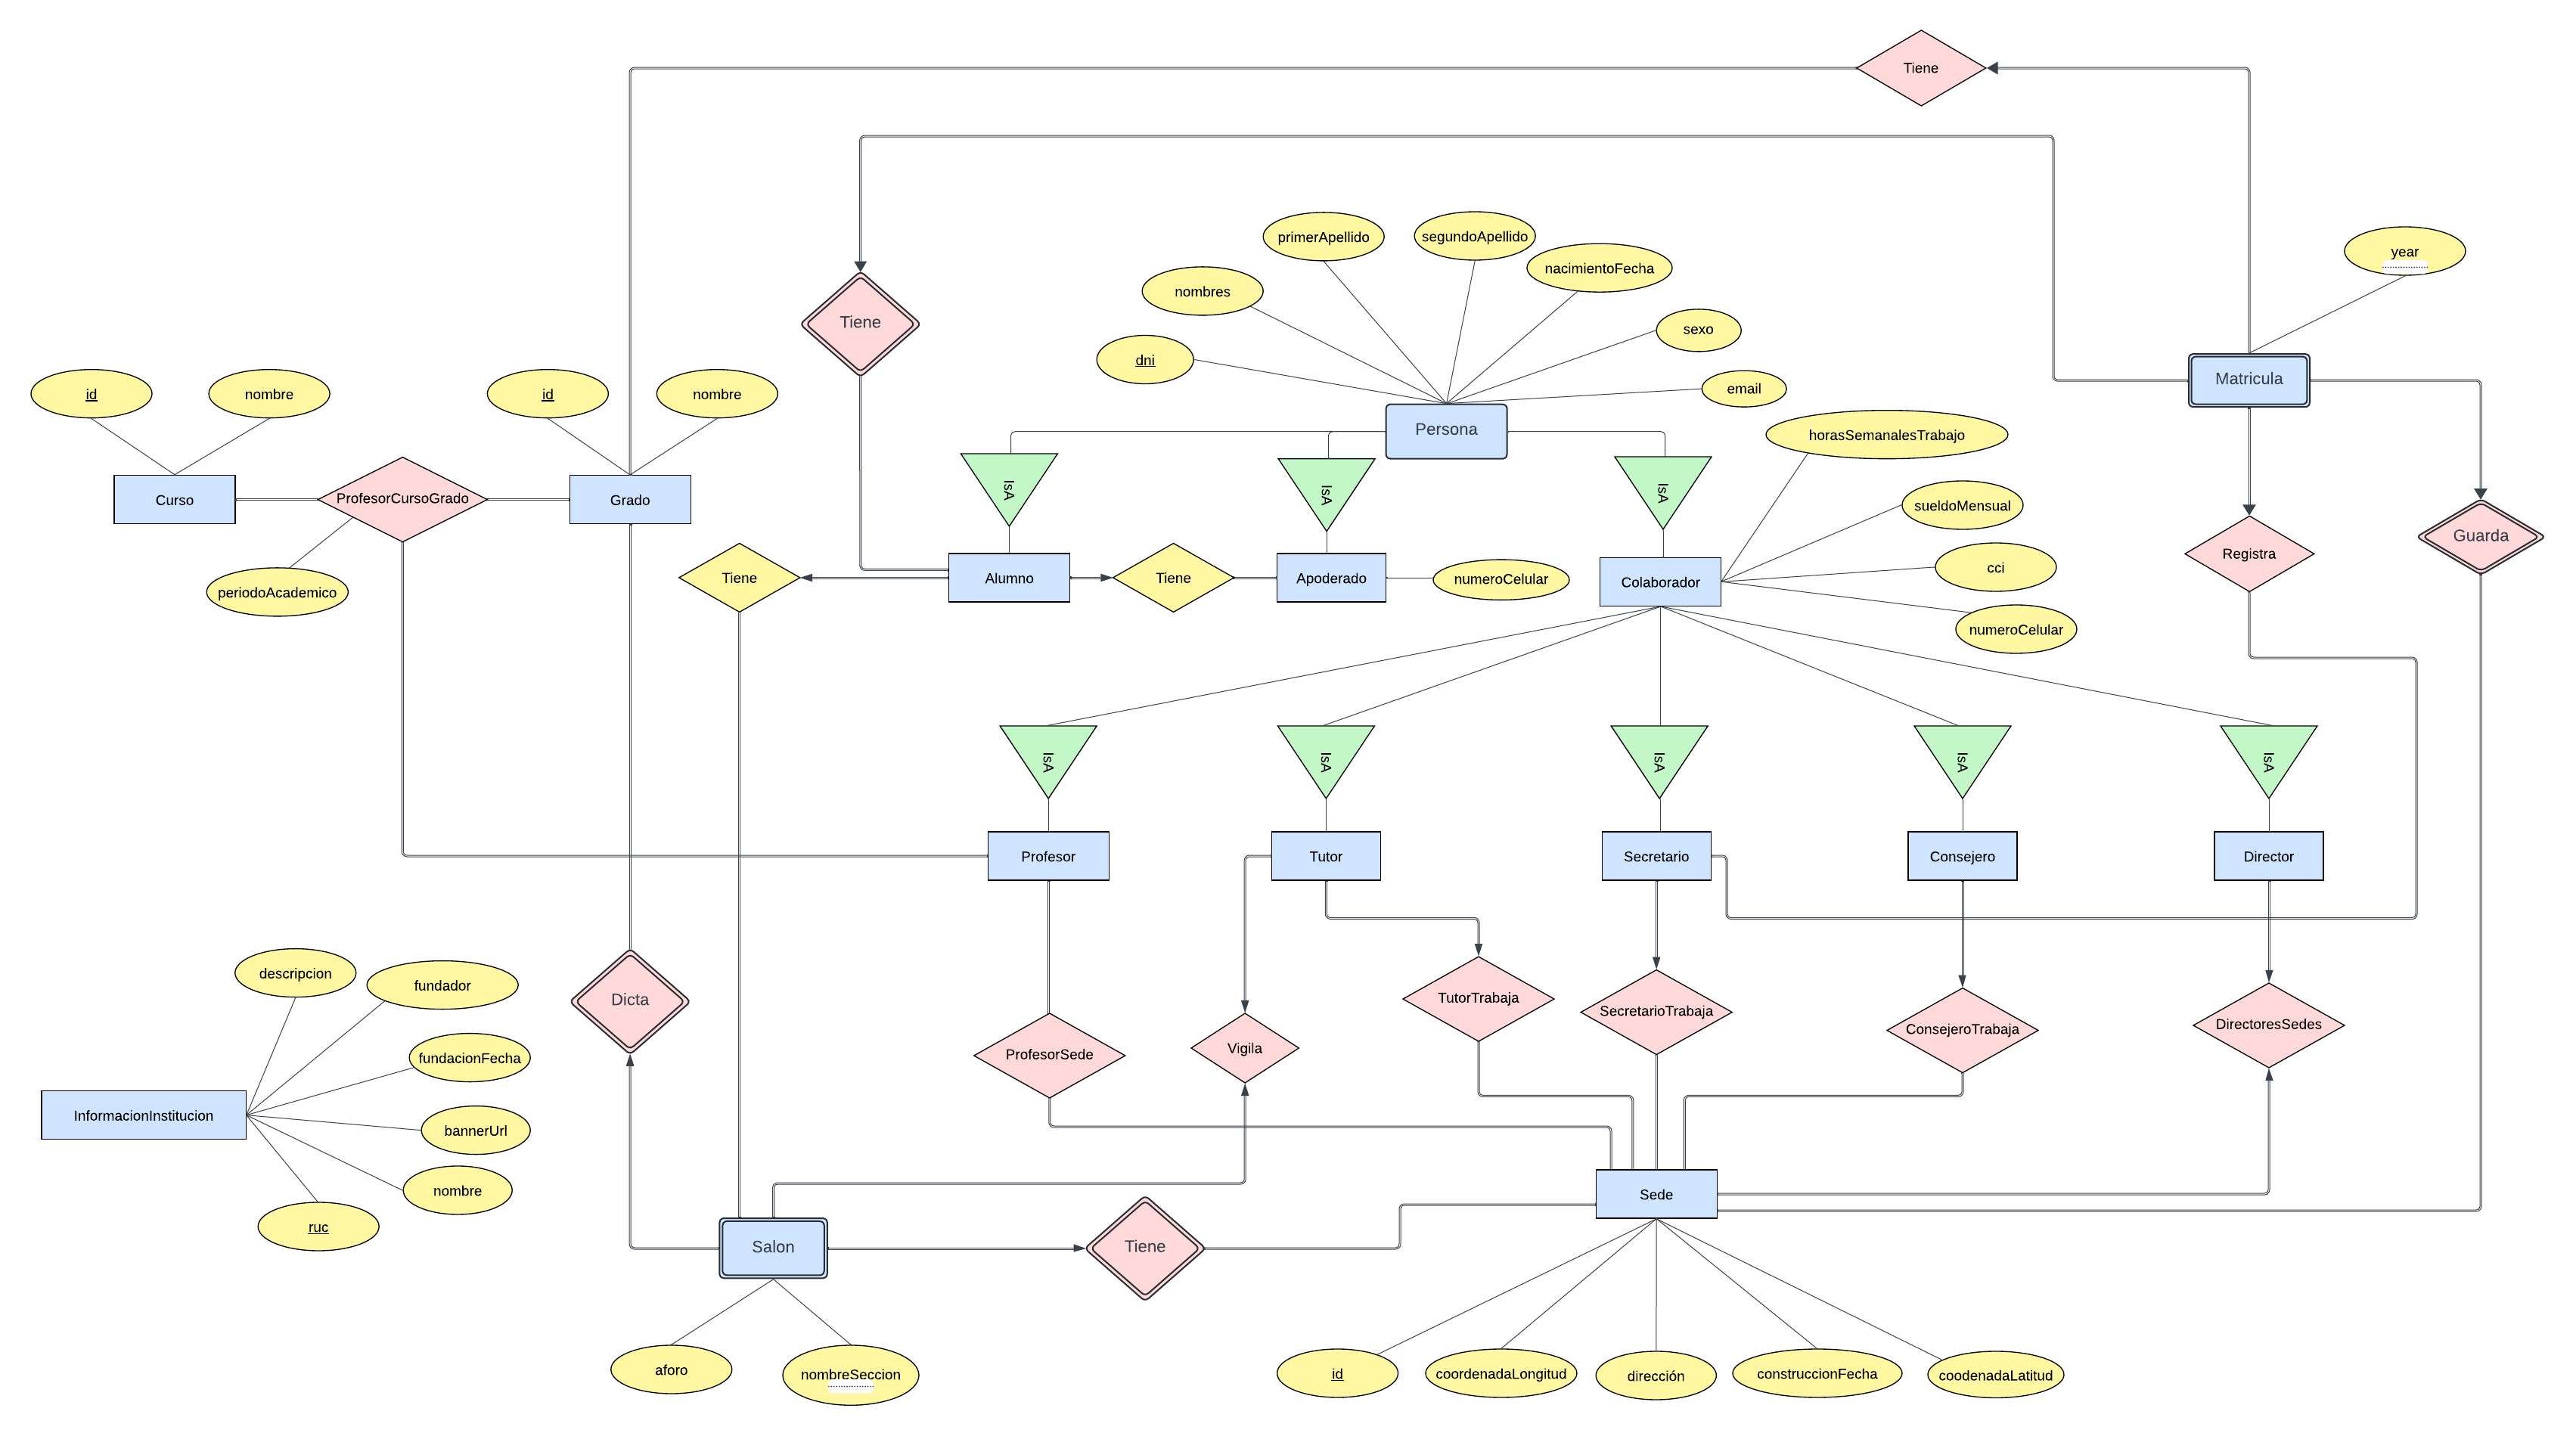
\includegraphics[width=\textwidth]{figures/modeloer.png}
	\caption{Modelo Entidad-Relación}
	\label{fig:my_label}
\end{figure}
\subsection{Especificaciones y consideraciones sobre el modelo}
\entidadBullets{Entidad InformacionInstitucion}{Almacena la información más importante de cada colegio: descripción, banner, nombre, fecha de fundación, fundador y el RUC como llave primaria.}{El RUC es seleccionado como la llave primaria ya que es un identificador único y oficial para cada institución. Esto facilita la gestión administrativa y legal de la información de la institución. Esta entidad no posee relaciones con ninguna otra entidad, ya que solo almacenerá una tupla la cual tendrá la información antes descrita.}
\entidadBullets{Entidad Persona}{Almacena la información más importante de cada individuo, incluyendo DNI (como llave primaria), nombres, apellidos, fecha de nacimiento, sexo y email.}{El DNI es usado como llave primaria, proporcionando un medio único y eficiente para identificar a cada persona. Esta entidad actúa como una superclase que hereda a las subclases Alumno, Apoderado y Colaborador, permitiendo solapamiento y cobertura total.}
\entidadBullets{Entidad Alumno}{Subclase de Persona. Está vinculado a un único salón y es matriculado por un solo apoderado.}{Hereda el DNI de Persona como llave primaria. La relación exclusiva con un apoderado y un salón justifica el mantenimiento de estas conexiones a través de claves foráneas, lo cual asegura integridad referencial y facilita consultas relacionales.}
\entidadBullets{Entidad Apoderado}{Subclase de Persona. Posee un número de celular adicional y puede matricular a uno o más alumnos.}{Utiliza el DNI de Persona como llave primaria. La capacidad de vincularse con múltiples alumnos refuerza su rol en el proceso educativo y administrativo, y la integridad referencial se mantiene a través de relaciones definidas en la base de datos.}
\entidadBullets{Entidad Colaborador}{Subclase de Persona. Incluye sueldo por hora, CCI, número de celular, horas semanales de trabajo y un atributo para saber si está activo o no.}{Continúa usando el DNI como llave primaria. Actúa como superclase para Profesor, Secretario, Director, Consejero, y Tutor, facilitando la implementación de políticas de empleo y administración dentro del colegio.}
\entidadBullets{Entidad Profesor}{Subclase de Colaborador. Puede enseñar en una o más sedes.}{Mantiene el DNI como llave primaria. La flexibilidad de enseñar en múltiples sedes es gestionada mediante una relación muchos a muchos con Sede, lo cual permite una programación eficiente.}
\entidadBullets{Entidad Secretario}{Secretario es una subclase de Colaborador y trabaja en una sola sede.}{El DNI es la llave primaria.Establece una relación muchos a uno con Sede la cual es justificada a través de una clave foránea, lo que garantiza que cada sede tenga un único secretario asociado.}
\entidadBullets{Entidad Director}{Director es una subclase de Colaborador y dirige una sola sede.}{El DNI es la llave primaria. La exclusividad de la relación uno a uno con Sede asegura un manejo claro de responsabilidades administrativas.}
\entidadBullets{Entidad Consejero}{Consejero es una subclase de Colaborador y trabaja en una sede.}{Utiliza el DNI como llave primaria. La relación muchos a uno con Sede facilita la asignación de responsabilidades y roles dentro del colegio y realiza la conexión a través de una llave foránea.}
\entidadBullets{Entidad Tutor}{Tutor es una subclase de Colaborador, trabaja en una sede y se le asigna un salón.}{El DNI como llave primaria, y sedeId como llave foránea, además su relación específica con un salón ayuda a mantener un control efectivo sobre el ambiente educativo.}
\entidadBullets{Entidad Sede}{Sede tiene un identificador único (ID), dirección, coordenadas y fecha de construcción. Está dirigida por un Director.}{El ID como llave primaria y el DNI del director como llave foránea.}
\entidadBullets{Entidad Salon}{Salón tiene como identificador nombreSeccion, tiene aforo, pertenece a una sede, en este se dictan clases de un grado y es supervisado por un Tutor.}{Tiene una llave primaria compuesta por los atributos nombreSeccion y sedeId lo que permite un manejo detallado de los espacios físicos. La relación con Tutor asegura supervisión directa y se relaciona mediante una llave foránea. Es considerada una entidad débil, ya que no podría existir un salón si es que no existe una sede al igual que no tendría sentido tener un salón sin que ninguna clase de algún grado se realice en él.}
\entidadBullets{Entidad Grado}{Grado está identificado por un ID y tiene un nombre. Contiene varios cursos y se enseña en varios salones.}{El ID como llave primaria facilita la organización de los programas educativos. Se relaciona con Profesor, Curso y Salón para estructurar el currículo.}
\entidadBullets{Entidad Curso}{Curso tiene un ID y un nombre, y está contenido en uno o más grados.}{El ID como llave primaria es adecuado para la gestión curricular. La relación con Grado y Profesor permite múltiples configuraciones pedagógicas.}
\entidadBullets{Entidad Matrícula}{Involucra Alumno, Apoderado, Grado, Sede y es realizada por un Secretario. Usa una clave primaria compuesta de alumnoDni, year, y sedeId.}{La clave primaria compuesta asegura una identificación única de cada registro, facilitando la administración y el seguimiento académico. Es una entidad débil, ya que para existir necesita que un apoderado matricule a un alumno con la ayuda de un secretario en cierto grado en cierta sede.}